\documentclass[fleqn]{exam}

\usepackage{fullpage}
\usepackage{enumerate}
% \usepackage{siunitx} 
\usepackage{unitsdef} 
\usepackage{graphicx}
\usepackage[fleqn]{mathtools}
\usepackage{cancel}
\usepackage{polynom}
\usepackage{float}
\usepackage{mdwlist}
\usepackage{booktabs}
\usepackage{cancel}
\usepackage{polynom}
\usepackage{caption}

\setlength{\mathindent}{.5 cm}

\everymath{\displaystyle}

% \begin{figure}[H]
%   \centering
%   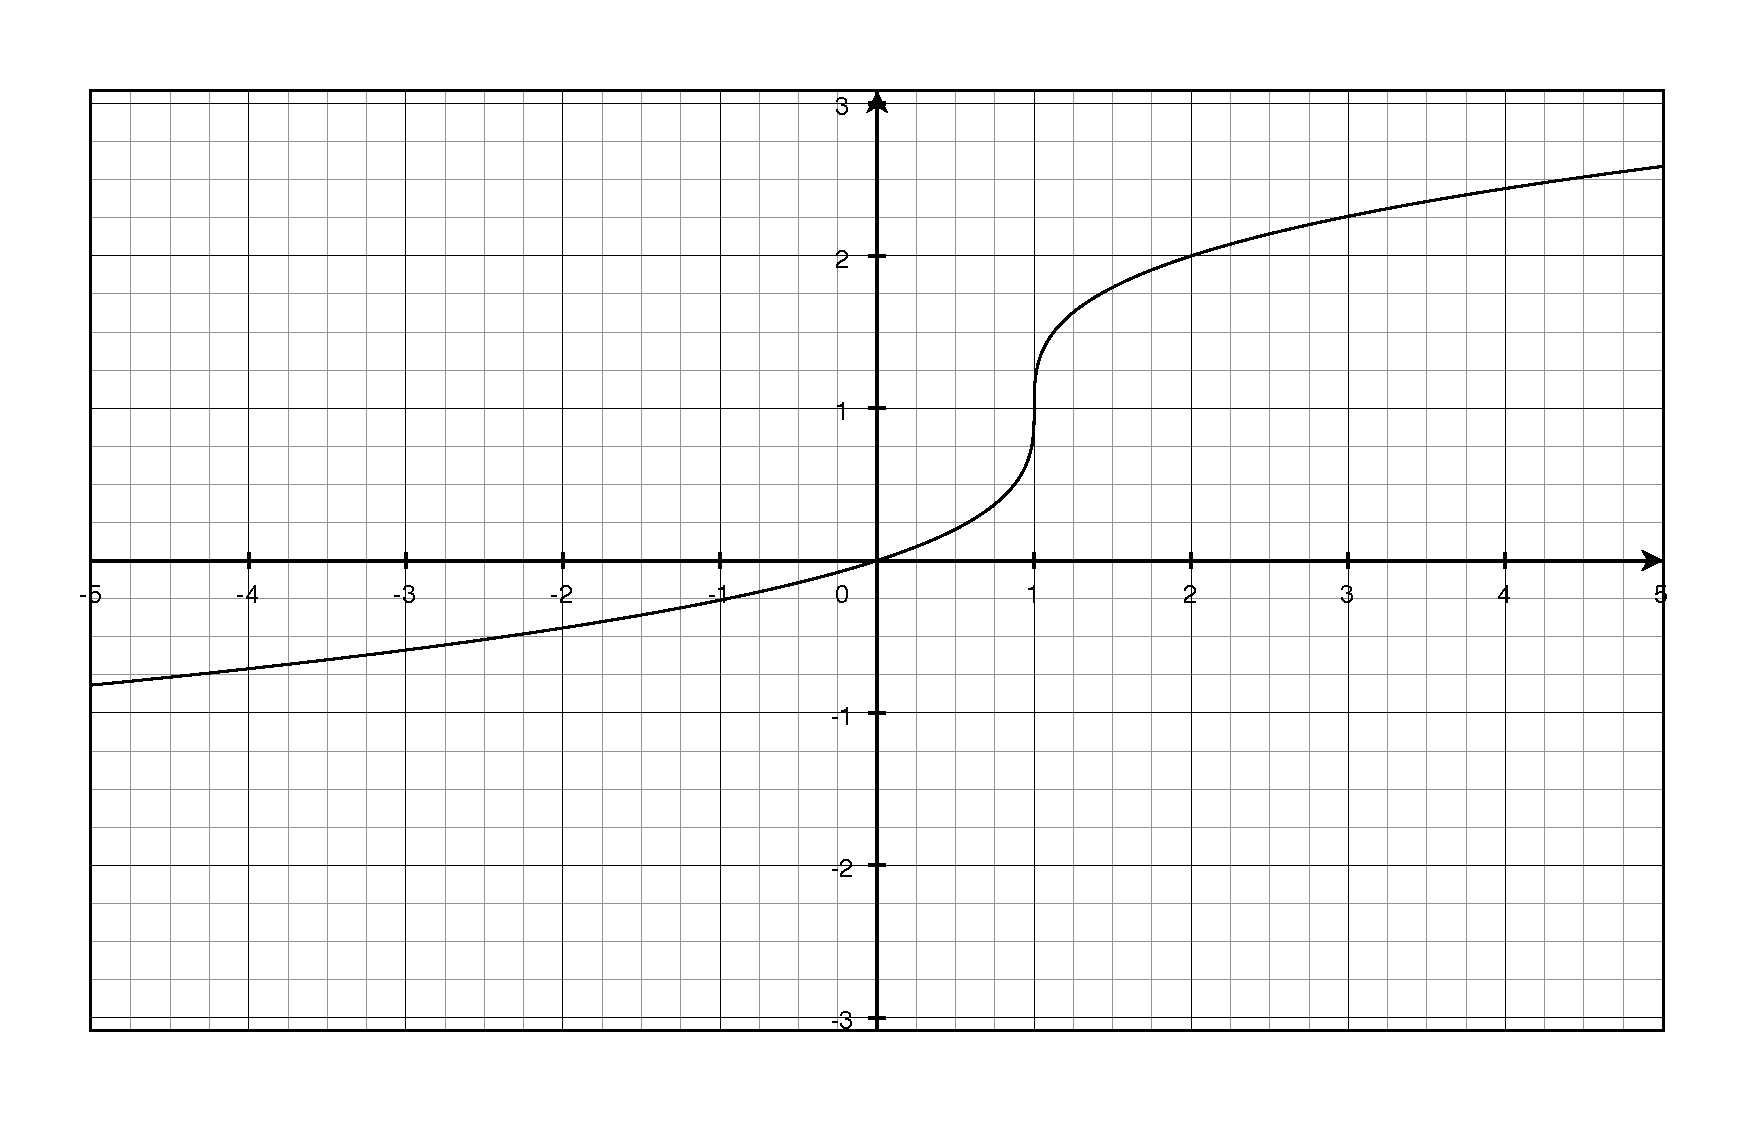
\includegraphics[scale=.3]{question7.eps}
%   \caption*{Question 7}
% \end{figure}

% \begin{tabular}{cc}
% \toprule
% period & amplitude \\
% \midrule
%   $\pi$ & $2$ \\
% \bottomrule
% \end{tabular}

\newunit{\inch}{in}
\newunit{\mile}{mile}
\newunit{\foot}{ft}
\newunit{\knot}{knot}
\newunit{\gallon}{gallon}

% \printanswers

\ifprintanswers 
\usepackage{2in1, lscape} 
\fi

\title{Math 263a \\ Chapters 2 and 3 Exam Study Guide}
\date{April 11, 2012}

\begin{document}

\maketitle

%% \section{General}
%% I tried to mention most of the key points in this sheet, but I may have missed a few.  A good way to prepare would be to
%% do the problems in the {\em Chapter Review} and {\em Sample Test} sections at the end of each of chapter.

\section{Limits and Continuity (Chapter 2)}

\subsection{Key Points}
\begin{itemize}
\item $\lim_{x \to c} f(x) = L$ means that when $x$ is near but different from $c$, then $f(x)$ is near $L$
\item Know the difference between right hand and left hand limits
\item Know how to find limits
\item You don't have to do $\epsilon/\delta$ proofs since these won't be on the final
\item A function is continuous at $c$ when $\lim_{x \to c} = f(c)$.  Of course if $f(c)$ is not defined, $f$ is not
  continuous at $c$.
\end{itemize}

\subsection{Sample Problems}
\begin{itemize}
\item $\lim_{x \to 0} \frac{x^2 - 4}{x+2}$
\item $\lim_{x \to 2} \frac{x^2 - 3x - 2}{x-2}$
\item $\lim_{x \to 3^+} \frac{\sqrt{x-3}}{x}$
\item Is $f(x) = \frac{x^2 - 9}{x-3}$ continuous at 3?
\item Where is $f(x) = \frac{2x + 7}{\sqrt{x + 5}}$ discontinuous?
\item Problems from {\em Chapter Review} and {\em Sample Test} from pp. 93-96
\end{itemize}

\pagebreak

\section{Derivatives (Chapter 3)}

\subsection{Key Points}
\begin{itemize}
\item The derivative of a function at a point is the slope of the function's tangent line at that point.
\item If $f$ is the amount of some quantity, $f'$ is the rate of change of that quantity.  For example, if $f$ is
  distance, $f'$ is velocity.
\item The definition of derivative is: $f'(x) = \lim_{h \to 0} \frac{f(x + h) - f(x)}{h}$.
\item Common notations for derivatives are: $f'$, $D_x$, $\frac{dy}{dx}$.
\item $D_x x^r = r x^{r - 1}$, where $r$ is any real number.
\item Know how to find derivatives of polynomials.
\item Know derivatives of sine, cosine, and tangent.  You can easily find the derivatives other trigonometric functions
  from these, if you need to.
\item Know the product rule, quotient rule, and chain rule
\item Know how to find higher-order derivatives and the notation for higher-order derivatives
\item Know how to find derivatives using implicit differentiation
\item Know how to solve related rates problems.  
\item Know how to do problems with differentials and approximations
\end{itemize}

\subsection{Sample Problems}

\begin{itemize}
\item
Find $f'(x)$:
\begin{itemize}
\item $f(x) = 4x^3 - 3x^2 + 2x - 6$
\item $f(x) = \sec^2 x$
\item $f(x) = \frac{x^2 + 1}{x^3 - 7x}$
\item $f(x) = \sin(\sqrt{x})$
\item $f(x) = x^2 \tan x$
\end{itemize}
\item $f(x) = 2x^7 - \pi^7 x + 17$; find $f'(x)$ and $f''(x)$ if 
\item $xy^2 + yx^2 = 1$; find $y'$ using implicit differentiation.
\item At noon, ship A is 100 km west of ship B.  Ship A is sailing east at 20 km/hr and ship B is sailing north at 25
  km/hr.  How fast is the distance between the ships changing at 4:00 PM?
\item If the radius of a sphere is $10 \pm .1 \cm$, what is the margin of error for the volume?
\item Problems from {\em Chapter Review} and {\em Sample Test} from pp. 168-170
\end{itemize}



\end{document}

